\documentclass[12pt,onecolumn,draftclsnofoot]{IEEEtran}
\usepackage[a4paper,margin=1in]{geometry}
\usepackage{times,graphicx,amsmath,booktabs,cite,url}
\usepackage[ruled,linesnumbered]{algorithm2e}
% additional packages (tables and the architecture diagram)
\usepackage{array,multirow,tabularx,amssymb}
\usepackage{tikz}
\usetikzlibrary{arrows.meta,positioning,fit,calc}
\graphicspath{{figures/}}
\urlstyle{same}
\newcolumntype{Y}{>{\raggedright\arraybackslash}X}% left-aligned table cells only (body text stays justified)
\newcolumntype{L}[1]{>{\raggedright\arraybackslash}p{#1}}

\begin{document}
\title{Patch-Ensemble FRQI and NEQR Quantum Kernels for Steel Surface Defect Classification}
\author{Group 02: Drishti (230527), Abhinav Singh (230528), Maheshwar Dwivedy, Kiran Khatter\\
School of Engineering \& Technology, BML Munjal University}
\maketitle

% ---------------------------------------------------------------- ABSTRACT
\begin{abstract}
Quantum image representations such as the Flexible Representation of Quantum Images (FRQI) and the Novel Enhanced Quantum Representation (NEQR) are commonly proposed as inputs to quantum classifiers, but when two images are compared through the overlap of their whole-image states, the similarity is computed pixel by pixel at fixed positions. Surface defects are textures whose position varies, and on the NEU-DET steel defect dataset such whole-image kernels reached only about 60\% accuracy in our earlier experiments. This paper proposes a patch-ensemble mixed-state kernel. Every small patch of an image is encoded with FRQI or NEQR, the image is represented by the uniform mixture of its patch states, and two images are compared through the Hilbert--Schmidt overlap $\mathrm{Tr}(\rho_A\rho_B)$, a quantity that a swap test can estimate directly. We evaluated 288 configurations (864 runs over three data splits) on a validation set only, froze the selected settings with cryptographic hashes and then tested each frozen model once on 360 held-out images. The FRQI model reaches $87.8\pm1.5\%$ accuracy and the NEQR model $82.7\pm10.1\%$, gains of 27.1 and 22.5 percentage points over the whole-image kernels (Holm-corrected $p<0.001$). A classical support vector machine on the same patches reaches $83.6\pm0.3\%$; it is not significantly different from FRQI ($p=0.060$), and a classical texture model remains best at $95.6\pm2.2\%$. The results show that the low accuracy of FRQI and NEQR kernels came from position-locked comparison rather than from the encodings, and that the improvement is not evidence of quantum advantage. All quantum computations were exact classical simulations.
\end{abstract}

\begin{IEEEkeywords}
FRQI, mixed-state quantum kernel, NEQR, quantum image representation, steel surface defect classification, swap test
\end{IEEEkeywords}

\noindent\textbf{Overleaf Project Link:} \url{https://www.overleaf.com/project/0123456789abcdef01234567}\\
\noindent\textbf{Code Repository:} \url{https://github.com/drishti55/Q-image/tree/v4-paper}

% ---------------------------------------------------------------- I. INTRODUCTION
\section{Introduction}
Machine learning on quantum computers has attracted attention because quantum states live in very large Hilbert spaces and may provide feature maps that are hard to compute classically \cite{biamonte2017,havlicek2019}. Current devices are small and noisy \cite{preskill2018}, so most practical studies use short circuits, a few qubits and classical simulation. Images are a natural test case, since many industrial inspection tasks are image-based and because a dedicated line of research describes how pixel positions and intensities can be stored in qubits \cite{yan2016survey}. Steel surface inspection is one such task: defects such as scratches, inclusions and rolled-in scale must be recognised quickly and reliably on production lines, and the NEU surface defect database provides a public benchmark for it \cite{song2013neu,he2020neudet}. Testing quantum methods on such data is useful even before large quantum computers exist, because it shows which encodings carry the information that real tasks need and which design decisions waste the few qubits available.

The two most widely used quantum image representations are FRQI \cite{le2011frqi}, which stores each intensity in the rotation angle of one colour qubit, and NEQR \cite{zhang2013neqr}, which stores a binary intensity code in several colour qubits. A simple way to use them for classification is as a quantum kernel \cite{schuld2019feature,havlicek2019}: the similarity of two images is the squared overlap of their encoded states, and a support vector machine (SVM) \cite{cortes1995} is trained on these similarities. The difficulty is that this overlap pairs pixel $i$ of one image with pixel $i$ of the other. A scratch that is shifted by a few pixels gives an almost unrelated state, while defect classes are defined by texture rather than by position. In our own earlier protocols, whole-image FRQI and NEQR kernels stayed at about 60\% accuracy on six NEU-DET classes, although classical texture features classified the same images at above 95\%. Re-tuning the encoding parameters did not help. For a researcher who wants to use quantum image encodings on inspection data, this leaves an open question: are the encodings themselves unsuitable, or is the way images are compared the problem?

Existing work does not resolve this. Studies of FRQI and NEQR focus on state preparation, storage and image operations rather than on classification of real textured images \cite{le2011frqi,zhang2013neqr,yan2016survey}. Quantum kernel and quantum convolution studies usually use synthetic data or handwritten digits \cite{havlicek2019,henderson2020quanv}, and recent theory warns that kernels on large registers concentrate and that classical models given the same data can often match quantum ones \cite{thanasilp2024,huang2021power}. Few studies compare a quantum image kernel with a classical model that receives exactly the same input, and few protect the test set against repeated use during model selection.

This paper addresses two research questions. \textbf{RQ1:} Does representing an image as the mixed state of its FRQI- or NEQR-encoded patches improve locked-test accuracy compared with whole-image FRQI and NEQR kernels? \textbf{RQ2:} Is the improvement due to the quantum encoding, that is, does the patch-ensemble quantum kernel outperform a classical model on the same patches and the best classical texture model?

The contributions of this work are as follows.
\begin{itemize}
\item A patch-ensemble mixed-state kernel for FRQI and NEQR, in which the number of qubits depends on the patch size rather than the image size, and whose kernel value can be estimated with a swap test.
\item A leakage-controlled evaluation on NEU-DET: 864 validation runs, a hash-frozen selection, a single locked-test evaluation per model and eight pre-declared, Holm-corrected statistical comparisons.
\item A matched classical control and an ablation study that separate the effect of patching from the effect of the quantum encoding.
\item A reconstruction study of all 1,800 images with 20 encodings built from real Qiskit circuits, released with the code and an interactive dashboard.
\end{itemize}

The rest of the paper is organised as follows: Section~II reviews related work, Section~III gives the background and problem formulation, Section~IV describes the method, Section~V the experimental setup, Section~VI the results, Section~VII the discussion and Section~VIII the conclusions.

% ---------------------------------------------------------------- II. RELATED WORK
\section{Related Work}
\subsection{Quantum image representations}
Le \emph{et al.} \cite{le2011frqi} introduced FRQI, which encodes an image of $N$ pixels in $\log_2 N+1$ qubits: a position register in uniform superposition and a single colour qubit rotated by an angle proportional to the intensity. Its main strengths are compactness and a preparation circuit built from controlled rotations, but intensities can only be recovered statistically from many measurements. NEQR \cite{zhang2013neqr} replaces the angle with a $q$-bit binary code, so that intensities can be read out exactly, at the cost of $q-1$ extra qubits and many multi-controlled gates. The survey by Yan \emph{et al.} \cite{yan2016survey} lists many variants that trade qubits against precision. These papers mainly study preparation complexity and image operations such as geometric transforms; they rarely evaluate whether the encodings are useful for classifying real images, which is the question we ask. The preparation cost is also significant in practice: an FRQI circuit needs one multi-controlled rotation per pixel, so its gate count grows quickly with image size. Our measurements confirm this, with more than 8,000 transpiled gates for a single $8\times8$ patch. Encoding a full $200\times200$ NEU image in this way is far beyond current devices, which is one reason to work with small patches.

\subsection{Quantum kernels and their limits}
Havl\'{i}\v{c}ek \emph{et al.} \cite{havlicek2019} and Schuld and Killoran \cite{schuld2019feature} showed that a quantum circuit that maps data to a state defines a kernel, which a classical SVM can use. Schuld \cite{schuld2021kernel} later argued that most supervised quantum models are in fact kernel methods. The demonstrations in these works used small synthetic data sets designed for the feature map. Huang \emph{et al.} \cite{huang2021power} showed that classical learners with access to the same data can often match quantum kernels, and Thanasilp \emph{et al.} \cite{thanasilp2024} proved that kernel values on large registers concentrate exponentially around a fixed value, making them hard to estimate with finite shots. Both results motivate our use of small patch registers and of a matched classical control. A further practical point is that many fidelity kernels behave like a very narrow similarity function: two inputs that differ slightly already have almost orthogonal states, and the kernel matrix approaches the identity. Scaling the input angles is one way to control this width, and our FRQI angle scale $b$ plays that role. Most published kernel experiments also report results on a single split and select hyper-parameters with the same data used for the final score, which makes small differences between quantum and classical models hard to interpret.

\subsection{Variational and convolution-style quantum models}
Variational quantum algorithms \cite{cerezo2021vqa} train parameterised circuits by classical optimisation, but they suffer from barren plateaus, where gradients vanish as circuits grow \cite{mcclean2018barren}. Henderson \emph{et al.} \cite{henderson2020quanv} applied small random quantum circuits to local image patches (quanvolution) and found performance similar to classical networks with comparable random non-linear layers. Our method shares the idea of processing local patches with small circuits, but it uses fixed, interpretable FRQI and NEQR encodings and a kernel instead of a trained network. A difference is how patch outputs are combined: quanvolution keeps the spatial map of patch outputs and passes it to a classical network, whereas we discard patch positions on purpose by averaging the patch states, which makes the representation tolerant to shifts.

\subsection{Steel surface defect recognition}
Song and Yan \cite{song2013neu} published the NEU database and classified it with noise-robust completed local binary patterns; He \emph{et al.} \cite{he2020neudet} added bounding-box annotations (NEU-DET) and an end-to-end convolutional detector. Classical texture descriptors such as local binary patterns \cite{ojala2002lbp} and grey-level co-occurrence matrices \cite{haralick1973glcm} remain strong baselines on this data, and one of them serves as our strongest classical reference. These descriptors summarise how often local intensity patterns occur in an image, independently of where they occur. The patch-ensemble kernel follows the same principle, but measures the similarity of local patterns through the overlap of their quantum states.

\subsection{Comparison and research gap}
Table~\ref{tab:related} compares eight key papers. Work on quantum image representations does not test classification on real textured images. Work on quantum kernels uses synthetic data, and work on steel defects is purely classical. None of these papers gives a matched classical control on the same input or a locked test set. Our work fills this gap: it asks whether FRQI and NEQR can classify a real defect data set when images are compared in a translation-tolerant way, and it measures how much of any gain is due to the quantum encoding.

\begin{table}[!t]
\centering
\caption{Comparison of key related work}
\label{tab:related}
\renewcommand{\baselinestretch}{1.1}\footnotesize
\begin{tabularx}{\linewidth}{@{}L{1.6cm}L{2.1cm}L{1.6cm}YYL{2.1cm}@{}}
\toprule
Paper & Method & Data & Key result & Limitation & Relevance here\\
\midrule
Le \emph{et al.} \cite{le2011frqi} & FRQI angle encoding & Illustrative images & Compact $\log_2N{+}1$-qubit encoding with polynomial preparation & Statistical read-out; no classification study & Encoding used in our kernel\\
Zhang \emph{et al.} \cite{zhang2013neqr} & NEQR basis encoding & Illustrative images & Exact intensity retrieval, simpler image operations & $q$ colour qubits; costly multi-controlled gates & Second encoding we compare\\
Havl\'{i}\v{c}ek \emph{et al.} \cite{havlicek2019} & Quantum kernel and variational classifier on hardware & Synthetic 2-D data & High accuracy on data built for the feature map & Toy data; no real images & Kernel framework we adopt\\
Schuld \& Killoran \cite{schuld2019feature} & Feature Hilbert-space view of QML & Small demos & Encodings define kernels usable by SVMs & No large-scale evaluation & Theoretical basis\\
Huang \emph{et al.} \cite{huang2021power} & Classical vs.\ quantum kernels with data & Engineered labels on real data & Classical models often match quantum ones & Advantage only on specially built tasks & Motivates our matched control\\
Thanasilp \emph{et al.} \cite{thanasilp2024} & Analysis of kernel concentration & Theory, numerics & Kernel values concentrate on large registers & Generic encodings & Motivates small patch registers\\
Henderson \emph{et al.} \cite{henderson2020quanv} & Quanvolution on image patches & MNIST & Similar to classical random-feature layers & Small digits data; no advantage & Patch-wise quantum processing\\
Song \& Yan \cite{song2013neu} & Completed LBP texture features & NEU (6 classes) & High accuracy, robust to noise & Classical, hand-crafted features & Data set and texture baseline\\
\bottomrule
\end{tabularx}
\end{table}

% ---------------------------------------------------------------- III. BACKGROUND
\section{Background and Problem Formulation}
\subsection{FRQI and NEQR}
Consider a patch of $N=2^n\times2^n$ pixels with intensities $x_i\in[0,1]$, where $i$ indexes the position. FRQI uses $2n$ position qubits and one colour qubit,
\begin{equation}
|\psi_{\mathrm{FRQI}}\rangle=\frac{1}{\sqrt N}\sum_{i=0}^{N-1}\big(\cos\theta_i|0\rangle+\sin\theta_i|1\rangle\big)\otimes|i\rangle,\qquad \theta_i=\frac{\pi}{2}\,b\,x_i,
\label{eq:frqi}
\end{equation}
where $b$ is an angle-scale parameter ($b=1$ is the original definition \cite{le2011frqi}). NEQR \cite{zhang2013neqr} uses $q$ colour qubits that hold the quantised intensity $c_i$:
\begin{equation}
|\psi_{\mathrm{NEQR}}\rangle=\frac{1}{\sqrt N}\sum_{i=0}^{N-1}|c_i\rangle\otimes|i\rangle,\qquad c_i=\mathrm{round}\big(x_i(2^q-1)\big).
\label{eq:neqr}
\end{equation}
FRQI therefore needs $2n+1$ qubits and NEQR $2n+q$ qubits. For two FRQI states of the same size, the overlap is $\langle\psi^A|\psi^B\rangle=\frac1N\sum_i\cos(\theta^A_i-\theta^B_i)$; it compares pixels at the same index only.

\subsection{Mixed states and the swap test}
A mixed state $\rho=\sum_k w_k|\psi_k\rangle\langle\psi_k|$ describes a system that is in state $|\psi_k\rangle$ with probability $w_k$. The swap test \cite{buhrman2001} applies a Hadamard gate, a controlled swap of two registers and another Hadamard gate to an ancilla qubit; the ancilla is measured as 0 with probability
\begin{equation}
\Pr[0]=\tfrac12\big(1+\mathrm{Tr}(\rho\sigma)\big),
\label{eq:swap}
\end{equation}
for any two input states $\rho$ and $\sigma$, pure or mixed. With $M$ repetitions, $\mathrm{Tr}(\rho\sigma)$ is estimated as $2\hat p_0-1$, where $\hat p_0$ is the observed fraction of zeros, and its standard error is $2\sqrt{p_0(1-p_0)/M}\le1/\sqrt M$. A useful special case is $\mathrm{Tr}(\rho^2)$, the purity of $\rho$, which equals 1 for a pure state and decreases as the mixture becomes more spread out; it appears on the diagonal of the kernel defined below. Table~\ref{tab:notation} summarises the notation used in the rest of the paper.

\begin{table}[!t]
\centering
\caption{Notation}
\label{tab:notation}
\renewcommand{\baselinestretch}{1.1}\footnotesize
\begin{tabular}{@{}ll@{\hspace{2em}}ll@{}}
\toprule
Symbol & Meaning & Symbol & Meaning\\
\midrule
$I$ & grayscale image, resized to $S\times S$ & $|\psi_k\rangle$ & encoded state of patch $k$\\
$p,\ s$ & patch side and stride (pixels) & $\rho_I$ & mixed state of image $I$\\
$P$ & number of patches per image & $D$ & dimension of a patch state, $2^{\text{qubits}}$\\
$x_i$ & intensity of pixel $i$ in $[0,1]$ & $K(A,B)$ & kernel between images $A$ and $B$\\
$b$ & FRQI angle scale & $C$ & SVM regularisation parameter\\
$q$ & NEQR bits per intensity & $y\in\mathcal Y$ & class label, $|\mathcal Y|=6$\\
\bottomrule
\end{tabular}
\end{table}

\subsection{Problem formulation}
The input is a grayscale image $I$ of a steel surface and the output is one of six defect classes $\mathcal Y=\{$crazing, inclusion, patches, pitted surface, rolled-in scale, scratches$\}$. Given a labelled training set $\{(I_j,y_j)\}$, the goal is a classifier $f(I)\in\mathcal Y$ that maximises accuracy and macro-averaged F1 on unseen images. We assume one defect class per image and use the official NEU-DET folders. Constraints are that every quantum register has at most 8 qubits, that models are chosen without access to the test images, and that each frozen model is tested once. Defect localisation, noise models, real quantum hardware and claims of quantum computational advantage are out of scope.

% ---------------------------------------------------------------- IV. METHODOLOGY
\section{Proposed Methodology}
\subsection{System architecture}
Fig.~\ref{fig:arch} shows the components of the system. A data module reads NEU-DET, fixes the splits in a hashed manifest and caches the resized images. The preprocessing module resizes, optionally stretches and cuts every image into patches. The quantum encoding module builds the FRQI or NEQR circuit of each patch in Qiskit \cite{qiskit2024} and obtains its statevector. The mixed-state module averages the patch states, and the kernel engine computes $\mathrm{Tr}(\rho_A\rho_B)$ for every pair of images. A precomputed-kernel SVM makes the prediction. A separate evaluation module performs validation-only selection, freezing, the single test evaluation and the statistics; a reconstruction module and a web dashboard reuse the same encoders.

\begin{figure}[!t]
\centering
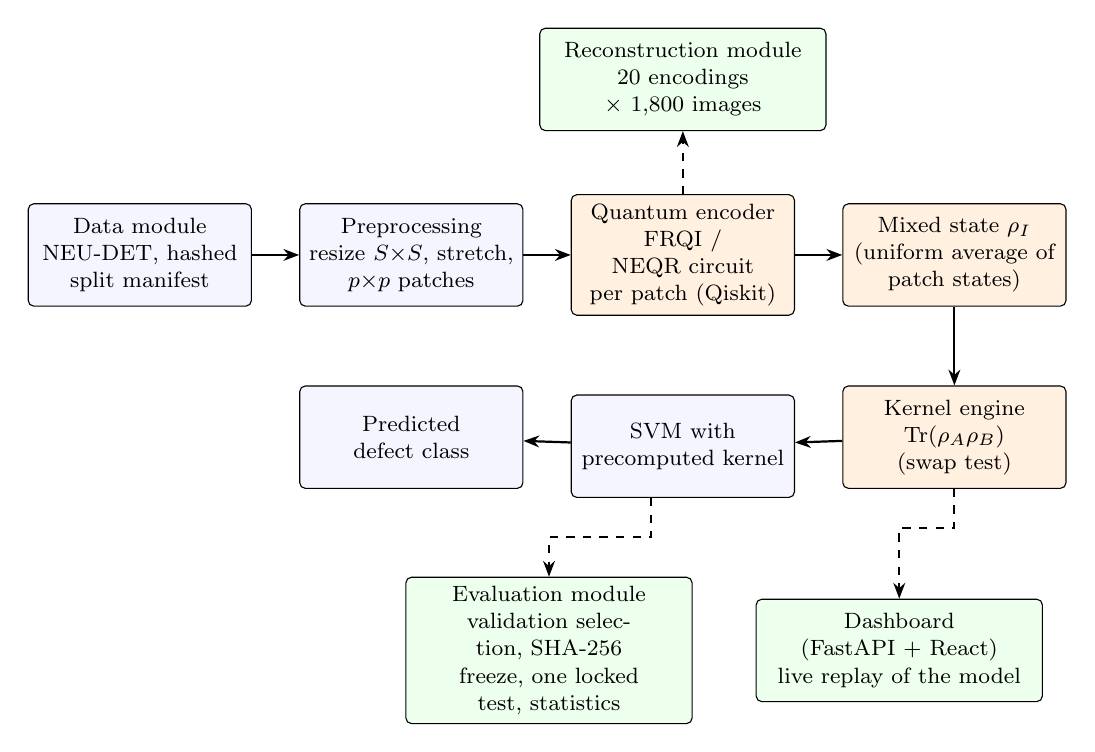
\begin{tikzpicture}[
  node distance=6mm and 6mm,
  every node/.append style={execute at begin node=\setlength{\baselineskip}{1.15em}},
  box/.style={draw, rounded corners=2pt, align=center, font=\footnotesize, minimum height=13mm, text width=26mm, fill=blue!4},
  qbox/.style={box, fill=orange!12},
  ebox/.style={box, fill=green!7, text width=34mm},
  arr/.style={-{Stealth[length=2mm]}, thick}]
\node[box] (data) {Data module\\ NEU-DET, hashed\\ split manifest};
\node[box, right=of data] (pre) {Preprocessing\\ resize $S{\times}S$, stretch,\\ $p{\times}p$ patches};
\node[qbox, right=of pre] (enc) {Quantum encoder\\ FRQI / NEQR circuit\\ per patch (Qiskit)};
\node[qbox, right=of enc] (mix) {Mixed state $\rho_I$\\ (uniform average of\\ patch states)};
\node[qbox, below=10mm of mix] (ker) {Kernel engine\\ $\mathrm{Tr}(\rho_A\rho_B)$\\ (swap test)};
\node[box, below=10mm of enc] (svm) {SVM with\\ precomputed kernel};
\node[box, below=10mm of pre] (out) {Predicted\\ defect class};
\node[ebox, above=8mm of enc] (rec) {Reconstruction module\\ 20 encodings $\times$ 1,800 images};
\node[ebox, below=10mm of svm, xshift=-17mm] (eval) {Evaluation module\\ validation selection, SHA-256\\ freeze, one locked test, statistics};
\node[ebox, right=8mm of eval] (dash) {Dashboard (FastAPI + React)\\ live replay of the model};
\draw[arr] (data) -- (pre); \draw[arr] (pre) -- (enc); \draw[arr] (enc) -- (mix);
\draw[arr] (mix) -- (ker); \draw[arr] (ker) -- (svm); \draw[arr] (svm) -- (out);
\draw[arr, dashed] (enc) -- (rec);
\draw[arr, dashed] (svm.south) ++(-4mm,0) -- ++(0,-5mm) -| (eval.north);
\draw[arr, dashed] (ker.south) -- ++(0,-5mm) -| (dash.north);
\end{tikzpicture}
\caption{Architecture of the proposed system. Solid arrows show the classification path for one image; dashed arrows show modules that reuse its outputs. Orange blocks contain the quantum part, which is simulated exactly on a CPU.}
\label{fig:arch}
\end{figure}

\subsection{Workflow}
Fig.~\ref{fig:workflow} shows the step-by-step flow. Panel (a) is the data protocol: candidates are trained and scored on the validation split, the best configuration per group is selected and hashed, and only then is the locked test set read, once per frozen model. Panel (b) is the path of one image through the kernel: patches, patch states, the mixed state $\rho$ and the kernel row passed to the SVM.

\begin{figure}[!t]
\centering
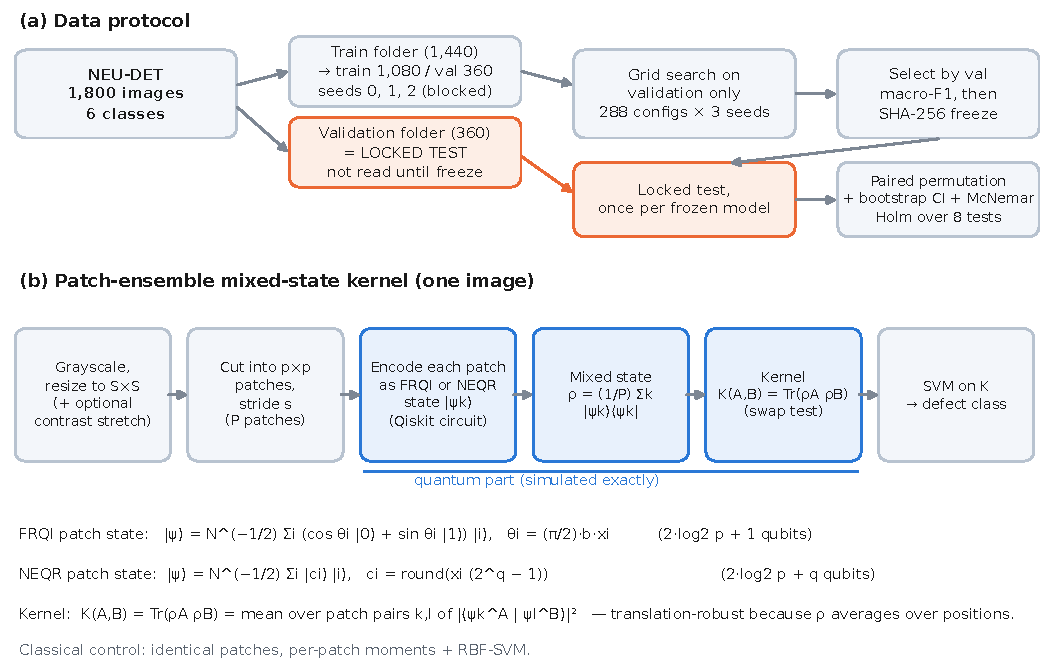
\includegraphics[width=\linewidth]{Fig01_methodology_flowchart.pdf}
\caption{Workflow. (a) Leakage-controlled protocol: validation-only selection, SHA-256 freeze, one locked-test evaluation per frozen model and pre-declared statistics. (b) Patch-ensemble mixed-state kernel for one image.}
\label{fig:workflow}
\end{figure}

\subsection{Preprocessing and patch extraction}
Each image is converted to grayscale, resized to $S\times S$ pixels with $S\in\{32,64,128\}$ and scaled to $[0,1]$. An optional per-image contrast stretch
\begin{equation}
x_i'=\frac{x_i-\min_j x_j}{\max_j x_j-\min_j x_j}
\label{eq:stretch}
\end{equation}
uses only the image itself, so no statistics leak from other images. The image is then cut into $p\times p$ patches with stride $s$, giving
\begin{equation}
P=\Big(\frac{S-p}{s}+1\Big)^2
\label{eq:npatch}
\end{equation}
patches. The patch side $p$ is a power of two so that it maps directly onto a position register.

\subsection{Patch-ensemble mixed-state kernel}
Each patch $k$ is encoded as $|\psi_k\rangle$ with \eqref{eq:frqi} or \eqref{eq:neqr}. The image is represented by the uniform mixture of its patch states,
\begin{equation}
\rho_I=\frac1P\sum_{k=1}^{P}|\psi_k\rangle\langle\psi_k|,
\label{eq:rho}
\end{equation}
a $D\times D$ density matrix, where $D=2^{2\log_2p+1}$ for FRQI and $2^{2\log_2p+q}$ for NEQR. Two images are compared by the Hilbert--Schmidt inner product
\begin{equation}
K(A,B)=\mathrm{Tr}(\rho_A\rho_B)=\frac{1}{P_AP_B}\sum_{k=1}^{P_A}\sum_{l=1}^{P_B}\big|\langle\psi^A_k|\psi^B_l\rangle\big|^2 .
\label{eq:kernel}
\end{equation}
The kernel is the average squared overlap over all pairs of patches, so a texture element that appears anywhere in both images contributes, independently of its position. $K$ is positive semi-definite because it is an inner product of density matrices. By \eqref{eq:swap}, a swap test between a randomly drawn patch state of $A$ and one of $B$ estimates $K(A,B)$ without building $\rho$ explicitly. In this study, $\rho$ was computed exactly from the statevectors, and $K$ as the element-wise inner product of the two real matrices.

Fig.~\ref{fig:illustration} illustrates these steps on a real training image with the frozen FRQI settings. For a $64\times64$ image, $8\times8$ patches and stride 4, \eqref{eq:npatch} gives $P=225$ patches; each patch state has $2\cdot3+1=7$ qubits, so $\rho$ is a $128\times128$ matrix. For the NEQR model ($128\times128$ image, $4\times4$ patches, stride 4, $q=4$) there are $P=1{,}024$ patches of $2\cdot2+4=8$ qubits and $\rho$ is $256\times256$.

\begin{figure}[!t]
\centering
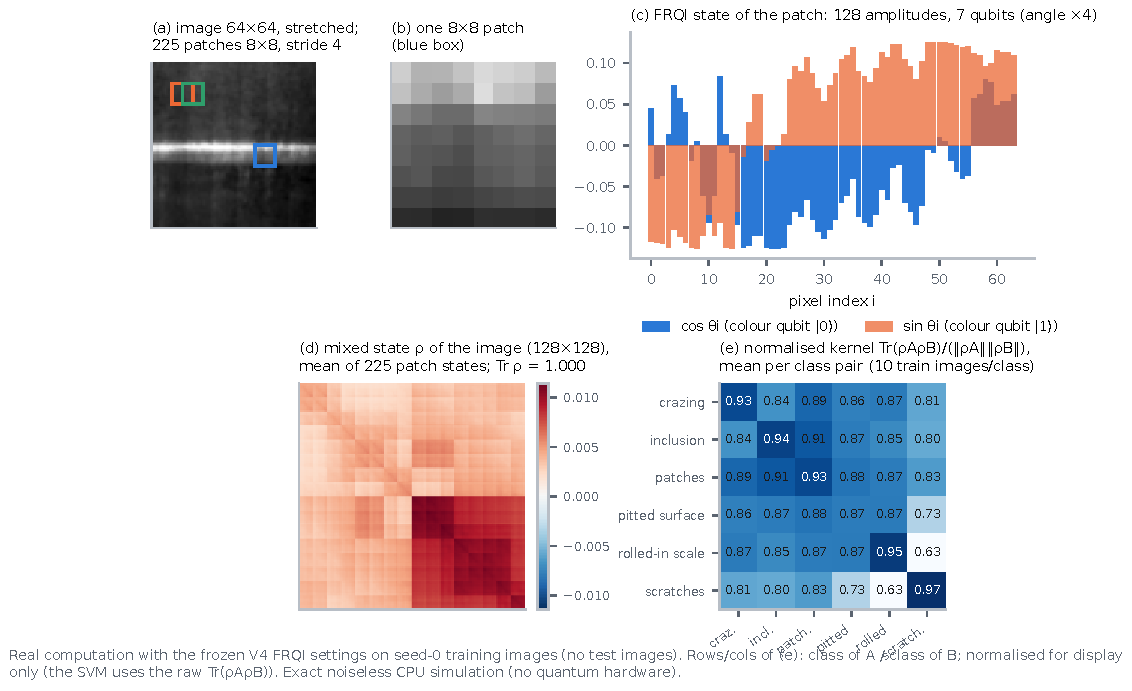
\includegraphics[width=\linewidth]{Fig02_patch_encoding_illustration.pdf}
\caption{The method on a real NEU-DET training image with the frozen FRQI settings ($64\times64$, $8\times8$ patches, stride 4): (a) image and example patches; (b) one patch; (c) its 7-qubit FRQI amplitudes; (d) the mixed state $\rho$ of the image; (e) kernel between classes for ten training images per class, normalised for display only.}
\label{fig:illustration}
\end{figure}

\subsection{Properties of the kernel}
\emph{Shift tolerance.} If the content of an image is shifted by a multiple of the stride, the interior patches are only re-ordered, and the uniform mixture in \eqref{eq:rho} does not depend on order; only patches at the border change. A whole-image kernel, in contrast, changes completely under the same shift.
\emph{Cost of exact simulation.} Computing all patch-pair overlaps in \eqref{eq:kernel} costs $O(P^2D)$ per image pair, while forming each $\rho$ once costs $O(PD^2)$ per image and each kernel entry then costs $O(D^2)$. Because $P^2\gg D$ here ($225^2$ versus 128 for FRQI), the density-matrix route is much cheaper, and it made the 864 validation runs feasible on a laptop.
\emph{Estimation on hardware.} If patch $k$ of $A$ and patch $l$ of $B$ are drawn uniformly at random, the expected swap-test outcome is exactly $K(A,B)$, so averaging single-shot swap tests over random patch pairs gives an unbiased estimate without ever preparing $\rho$ as a whole. The required register is two patch registers plus one ancilla.

\subsection{Classifier}
A multi-class SVM \cite{cortes1995} with a precomputed kernel (one-versus-one, scikit-learn \cite{pedregosa2011}) predicts
\begin{equation}
f(I)=\arg\max_{y\in\mathcal Y}\sum_{(u,v)\ni y}\mathbb 1\Big[\mathrm{sign}\Big(\sum_{j}\alpha^{uv}_jy^{uv}_jK(I_j,I)+\beta^{uv}\Big)\ \text{votes for } y\Big],
\label{eq:svm}
\end{equation}
where $\alpha^{uv}_j$ and $\beta^{uv}$ are the dual coefficients and bias of the binary SVM for classes $u$ and $v$, and $y^{uv}_j\in\{\pm1\}$. Algorithm~\ref{alg:kernel} summarises training and prediction, and Algorithm~\ref{alg:protocol} the evaluation protocol.

\begin{algorithm}[!t]
\caption{Patch-ensemble kernel classifier}
\label{alg:kernel}
\KwIn{training images $\{(I_j,y_j)\}_{j=1}^{n}$, query image $I_*$, encoding $E\in\{\text{FRQI},\text{NEQR}\}$, $S,p,s$, $b$ or $q$, stretch flag, $C$}
\KwOut{predicted class $\hat y_*$}
\ForEach{image $I\in\{I_1,\dots,I_n,I_*\}$}{
  resize $I$ to $S\times S$, scale to $[0,1]$, apply \eqref{eq:stretch} if the stretch flag is set\;
  extract the $P$ patches $\mathbf x_1,\dots,\mathbf x_P$ of side $p$ and stride $s$\;
  \For{$k\leftarrow1$ \KwTo $P$}{prepare $|\psi_k\rangle$ with encoder $E$ (\eqref{eq:frqi} or \eqref{eq:neqr})\;}
  $\rho_I\leftarrow\frac1P\sum_k|\psi_k\rangle\langle\psi_k|$\;
}
$K_{jj'}\leftarrow\mathrm{Tr}(\rho_{I_j}\rho_{I_{j'}})$ for all training pairs\;
train a one-vs-one SVM with precomputed kernel $K$ and parameter $C$\;
$\mathbf k_*\leftarrow[\mathrm{Tr}(\rho_{I_*}\rho_{I_j})]_{j=1}^{n}$\;
$\hat y_*\leftarrow$ SVM prediction for $\mathbf k_*$\;
\end{algorithm}

\begin{algorithm}[!t]
\caption{Leakage-controlled selection and evaluation}
\label{alg:protocol}
\KwIn{model groups $\mathcal G$, grid $\Theta_g$ per group, seeds $r\in\{0,1,2\}$, splits (train$_r$, val$_r$), locked test set $T$}
\KwOut{test metrics of one frozen configuration per group}
\ForEach{$g\in\mathcal G$, $\theta\in\Theta_g$, $r\in\{0,1,2\}$}{
  train with Algorithm~\ref{alg:kernel} on train$_r$; record macro-F1 on val$_r$\;
}
\ForEach{$g\in\mathcal G$}{$\theta_g^*\leftarrow\arg\max_\theta$ mean validation macro-F1 over seeds\;}
write the selections to disk and store their SHA-256 hashes\;
\ForEach{$g\in\mathcal G$}{
  abort if any selection hash has changed\;
  \For{$r\leftarrow0$ \KwTo $2$}{evaluate the saved model ($\theta_g^*$, train$_r$) on $T$ once; log the access\;}
}
run the eight pre-declared comparisons with Holm correction\;
\end{algorithm}

\subsection{Implementation and verification}
For speed, the patch states are computed from the closed-form amplitudes in \eqref{eq:frqi} and \eqref{eq:neqr} rather than by simulating every circuit for every patch. To make sure that this shortcut describes real circuits, the project builds the corresponding FRQI and NEQR encoder circuits in Qiskit, and a unit test checks, for both encodings and random images, that the kernel computed from the density matrices equals the mean squared overlap of the Qiskit statevectors. A second test shifts a random $16\times16$ image cyclically by one stride: the normalised patch-ensemble kernel between the original and the shifted image stays above 0.999, while the whole-image FRQI kernel drops below 0.95. The circuit resources reported in Section~VI are obtained by transpiling the same encoder circuits, so the qubit and gate counts refer to the circuits that a quantum device would run.

\subsection{Design choices}
\emph{Patches instead of whole images:} averaging over patches removes the dependence on absolute position, which is the main weakness of whole-image kernels, and keeps registers at 5--8 qubits, below the size where kernel concentration is expected \cite{thanasilp2024}. \emph{A uniform mixture instead of concatenation:} concatenating patch states would again fix positions; the mixture is the simplest position-free summary and is directly measurable with a swap test. \emph{A kernel SVM instead of a variational classifier:} kernels avoid barren plateaus \cite{mcclean2018barren} and give a convex training problem, and our earlier variational models were the weakest quantum models. \emph{An angle scale $b>1$:} with $b=1$, intensities only cover a quarter turn of the colour qubit and nearby textures give nearly identical overlaps; larger $b$ spreads them out. \emph{Per-image contrast stretch:} it removes global brightness differences between images without using any statistics from other images.

% ---------------------------------------------------------------- V. EXPERIMENTAL SETUP
\section{Experimental Setup}
\subsection{Data set and splits}
NEU-DET \cite{song2013neu,he2020neudet} contains 1,800 grayscale $200\times200$ images of hot-rolled steel strips, 300 per class. The 360 images of the official validation folder form the locked test set. The 1,440 images of the training folder are split into 1,080 training and 360 validation images by a group-blocked split (blocks of 20 consecutive indices, three validation blocks per class), so that near-duplicate neighbouring images do not fall into both sets. The split is repeated with three seeds (0, 1, 2); every split is balanced, as shown in Table~\ref{tab:data}. The split manifest is stored with its SHA-256 hash and shared by protocols V2, V3 and V4, so all baselines see exactly the same training, validation and test images. In every run, the kernel matrix between the 1,080 training images is computed, the SVM is fitted, and the 360 validation images are scored; the trained model is saved so that the test stage only applies it and never retrains.

\begin{table}[!t]
\centering
\caption{NEU-DET splits per class (identical for seeds 0, 1 and 2)}
\label{tab:data}
\renewcommand{\baselinestretch}{1.1}\footnotesize
\begin{tabularx}{\linewidth}{@{}Yrrrr@{}}
\toprule
Class & Train & Validation & Locked test & Total\\
\midrule
Each class (crazing, inclusion, patches, pitted surface, rolled-in scale, scratches) & 180 & 60 & 60 & 300\\
All six classes & 1,080 & 360 & 360 & 1,800\\
\bottomrule
\end{tabularx}
\end{table}

\subsection{Tools and platform}
The code is written in Python 3.11.0 with Qiskit 2.5.2 and Qiskit Aer 0.17.2 \cite{qiskit2024}, scikit-learn 1.9.1 \cite{pedregosa2011} and NumPy 2.4.6. All runs were performed on a laptop CPU (Apple M5, 16\,GB RAM); no GPU, quantum hardware or noise model was used. Circuit resources were obtained by transpiling the encoder circuits to the basis $\{\mathrm{cx},\mathrm{rz},\mathrm{sx},\mathrm{x}\}$ at optimisation level 1 with all-to-all connectivity.

\subsection{Baselines}
We compare against four baselines evaluated on the same splits and test images: (i) the whole-image FRQI kernel ($8\times8$ pixels, $b=2$) and (ii) the whole-image NEQR kernel ($16\times16$, 4 bits) from our earlier protocol (V2); (iii) a re-tuned whole-image FRQI kernel from protocol V3; (iv) a classical control that uses exactly the same patches but describes each image by the mean patch vector and the mean outer product of raw patch intensities (the classical analogue of $\rho$ without the quantum feature map), standardised and classified by an RBF-SVM; and (v) the best classical model of protocol V3, an RBF-SVM on 12 principal components of local binary pattern \cite{ojala2002lbp} and co-occurrence \cite{haralick1973glcm} texture features.

\subsection{Evaluation metrics}
\emph{Accuracy} is the headline metric because the test set is balanced. \emph{Macro-F1} weights all classes equally and was the selection criterion. \emph{Per-class F1} shows which defects fail. For each pre-declared comparison, per-image correctness is averaged over seeds and tested with a paired sign-flip permutation test (10,000 permutations); 95\% confidence intervals come from a paired bootstrap \cite{efron1993}, McNemar's test \cite{mcnemar1947} is reported per seed, and $p$-values are Holm-corrected over the eight comparisons \cite{holm1979}. Reconstruction quality is measured with the mean squared error (MSE) and SSIM \cite{wang2004ssim}.

\subsection{Parameters}
Table~\ref{tab:params} lists every setting. The grid gives 288 configurations, each trained with three seeds (864 runs, none failed). The selection rule, the eight comparisons and the choice of headline models were fixed before the test set was read.

\begin{table}[!t]
\centering
\caption{Search space and fixed settings (selected values in bold)}
\label{tab:params}
\renewcommand{\baselinestretch}{1.1}\footnotesize
\begin{tabularx}{\linewidth}{@{}L{3.3cm}Y@{}}
\toprule
Setting & Values\\
\midrule
FRQI, $4\times4$ patches & $S/s\in\{32/2,\ \mathbf{64/4}\}$; $b\in\{1,2,\mathbf 4\}$; stretch $\in\{$none, \textbf{on}$\}$; 48 configs\\
FRQI, $8\times8$ patches & $S/s\in\{32/4,\ \mathbf{64/4},\ 128/8\}$; $b\in\{1,2,\mathbf 4\}$; stretch $\in\{$none, \textbf{on}$\}$; 72 configs\\
NEQR, $2\times2$ patches & $S/s\in\{32/1,\ \mathbf{64/2}\}$; $q\in\{\mathbf4,5,6\}$; stretch $\in\{$\textbf{none}, on$\}$; 48 configs\\
NEQR, $4\times4$ patches & $S/s\in\{32/2,\ 64/4,\ \mathbf{128/4}\}$; $q\in\{3,\mathbf4\}$; stretch $\in\{$\textbf{none}, on$\}$; 48 configs\\
Classical patch control & $(S,p,s)\in\{(64,4,4),\ \mathbf{(64,8,4)},\ (128,4,4)\}$; $\gamma\in\{0.3,\mathbf1,3\}$ (divided by feature count); stretch $\in\{$none, \textbf{on}$\}$; 72 configs\\
SVM $C$ (all groups) & $\{1,10,100,\mathbf{1000}\}$\\
Seeds and runs & seeds 0, 1, 2; 288 configurations $\times$ 3 = 864 runs\\
Selection & maximum mean validation macro-F1 over seeds; ties broken by grid order\\
Headline models & FRQI and NEQR groups with the highest validation macro-F1 ($8\times8$ and $4\times4$ patches)\\
Statistics & 10,000 permutations; 10,000 bootstrap resamples; Holm over 8 tests; $\alpha=0.05$\\
Reconstruction & shots $\in\{100, 1\text{k}, 10\text{k}, 100\text{k}\}$ and exact statevector; 20 methods; all 1,800 images\\
\bottomrule
\end{tabularx}
\end{table}

% ---------------------------------------------------------------- VI. RESULTS
\section{Results and Analysis}
\subsection{RQ1: Improvement over whole-image kernels}
Table~\ref{tab:main} compares the patch-ensemble models with all baselines. The FRQI model with $8\times8$ patches reaches $87.8\pm1.5\%$ test accuracy and $87.5\pm1.6\%$ macro-F1, against $60.6\pm1.2\%$ for the whole-image FRQI kernel. The NEQR model with $4\times4$ patches reaches $82.7\pm10.1\%$, against $60.2\pm0.4\%$. Validation and test scores are close for FRQI (88.0 vs.\ 87.5 macro-F1), which indicates that its selection did not overfit the validation split; for NEQR the test score is lower and more variable.

\begin{table}[!t]
\centering
\caption{Locked-test results, mean $\pm$ s.d.\ over three seeds (360 images; F1 = macro-F1; best value per column in bold)}
\label{tab:main}
\renewcommand{\baselinestretch}{1.1}\footnotesize
\begin{tabular}{@{}llccc@{}}
\toprule
Model & Type & Val.\ F1 (\%) & Test acc.\ (\%) & Test F1 (\%)\\
\midrule
\textbf{Proposed:} FRQI, $8\times8$ patches & quantum (sim.) & 88.0 & $87.8\pm1.5$ & $87.5\pm1.6$\\
\textbf{Proposed:} NEQR, $4\times4$ patches & quantum (sim.) & 89.2 & $82.7\pm10.1$ & $80.4\pm13.5$\\
FRQI, $4\times4$ patches & quantum (sim.) & 85.7 & $85.3\pm1.7$ & $85.0\pm1.6$\\
NEQR, $2\times2$ patches & quantum (sim.) & 88.2 & $81.5\pm10.6$ & $79.2\pm14.1$\\
\midrule
Whole-image FRQI (V2) & quantum (sim.) & 69.3 & $60.6\pm1.2$ & $58.3\pm1.3$\\
Whole-image NEQR (V2) & quantum (sim.) & 72.7 & $60.2\pm0.4$ & $56.5\pm0.4$\\
Whole-image FRQI, re-tuned (V3) & quantum (sim.) & 69.4 & $57.5\pm2.1$ & $55.3\pm2.4$\\
Classical RBF-SVM, same patches & classical & 83.8 & $83.6\pm0.3$ & $83.3\pm0.3$\\
Classical texture RBF-SVM (V3) & classical & \textbf{95.3} & $\mathbf{95.6\pm2.2}$ & $\mathbf{95.5\pm2.2}$\\
\bottomrule
\end{tabular}
\end{table}

Fig.~\ref{fig:protocols} places these numbers in the history of the project. Both encodings stayed near 60\% in protocols V2 and V3, even after re-tuning, and jump to more than 80\% with the patch-ensemble kernel. This pattern suggests that the bottleneck was the position-locked comparison, not a poor choice of encoding parameters.

\begin{figure}[!t]
\centering
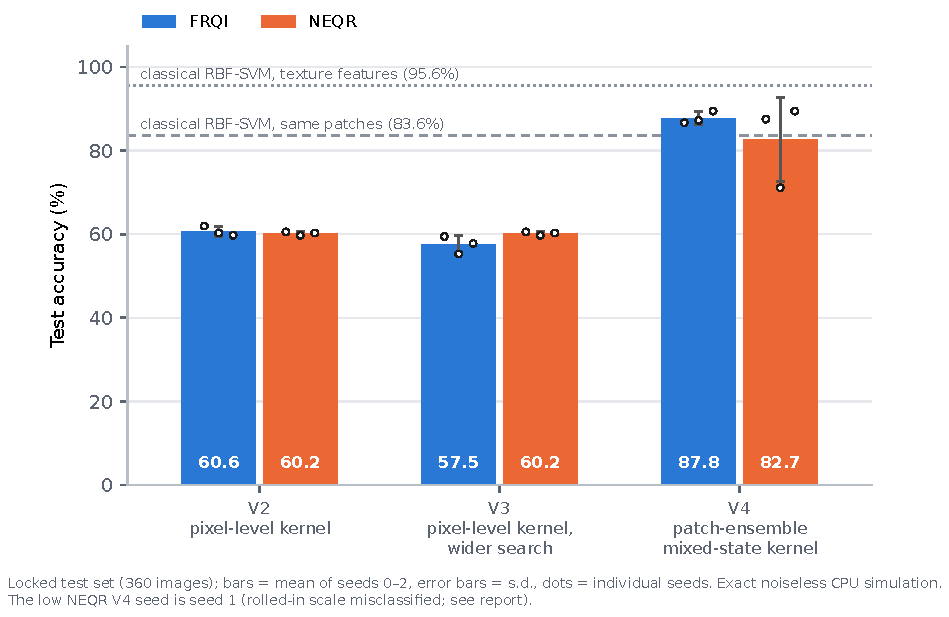
\includegraphics[width=0.85\linewidth]{Fig04_frqi_neqr_across_protocols.pdf}
\caption{Locked-test accuracy of FRQI and NEQR models across protocols V2, V3 and V4 (mean $\pm$ s.d.\ over three seeds); the dashed line marks chance level (16.7\%).}
\label{fig:protocols}
\end{figure}

Fig.~\ref{fig:forest} and Table~\ref{tab:stats} give the paired statistics. The FRQI gain over the V2 whole-image kernel is $+27.1$ percentage points (pp) with 95\% CI $[+21.7,+32.7]$, and over the re-tuned V3 kernel $+30.3$\,pp; the NEQR gain is $+22.5$\,pp $[+18.5,+26.7]$. All three are significant after Holm correction ($p<0.001$), and McNemar counts show far more images fixed than broken in every seed (for FRQI vs.\ V2, 114:25, 118:21 and 123:16). FRQI is also better than NEQR by $+5.1$\,pp ($p=0.045$). The answer to RQ1 is therefore yes, for both encodings.

\begin{figure}[!t]
\centering
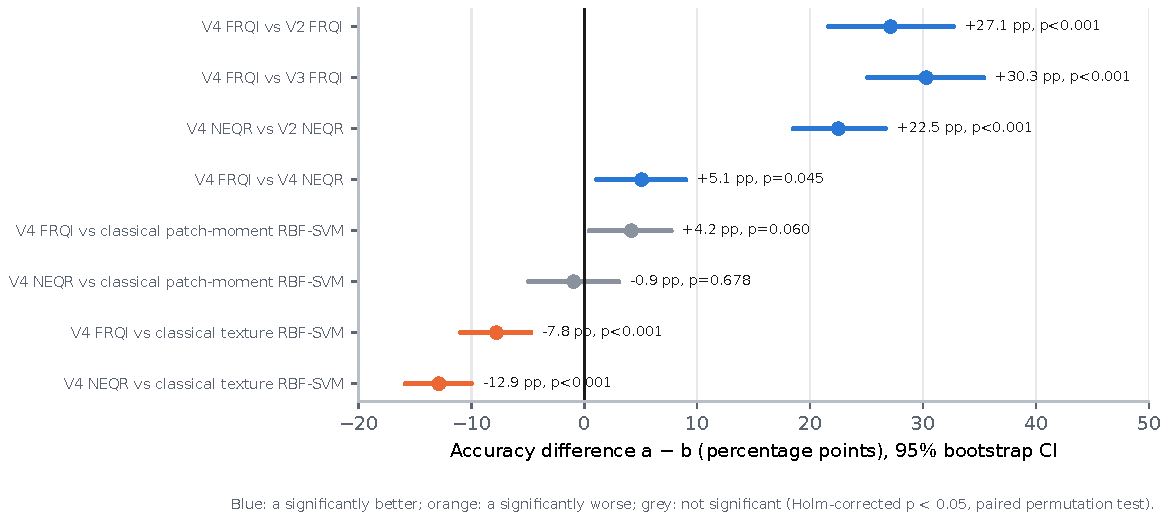
\includegraphics[width=\linewidth]{Fig05_comparisons_forest.pdf}
\caption{Accuracy differences of the eight pre-declared comparisons with paired-bootstrap 95\% confidence intervals and Holm-corrected $p$-values.}
\label{fig:forest}
\end{figure}

\begin{table}[!t]
\centering
\caption{Pre-declared paired comparisons (Holm-corrected over eight tests)}
\label{tab:stats}
\renewcommand{\baselinestretch}{1.1}\footnotesize
\begin{tabular}{@{}lrrcc@{}}
\toprule
Comparison (A vs.\ B) & $\Delta$ (pp) & 95\% CI (pp) & $p_{\text{Holm}}$ & Significant\\
\midrule
FRQI patches vs.\ whole-image FRQI (V2) & $+27.1$ & $[+21.7,+32.7]$ & $<0.001$ & yes\\
FRQI patches vs.\ whole-image FRQI (V3) & $+30.3$ & $[+25.1,+35.4]$ & $<0.001$ & yes\\
NEQR patches vs.\ whole-image NEQR (V2) & $+22.5$ & $[+18.5,+26.7]$ & $<0.001$ & yes\\
FRQI patches vs.\ NEQR patches & $+5.1$ & $[+1.1,+9.0]$ & 0.045 & yes\\
FRQI patches vs.\ classical, same patches & $+4.2$ & $[+0.5,+7.7]$ & 0.060 & no\\
NEQR patches vs.\ classical, same patches & $-0.9$ & $[-4.9,+3.1]$ & 0.678 & no\\
FRQI patches vs.\ classical texture SVM & $-7.8$ & $[-10.9,-4.7]$ & $<0.001$ & yes\\
NEQR patches vs.\ classical texture SVM & $-12.9$ & $[-15.8,-10.0]$ & $<0.001$ & yes\\
\bottomrule
\end{tabular}
\end{table}

\subsection{RQ2: Is the gain due to the quantum encoding?}
On identical patches, the classical control reaches $83.6\pm0.3\%$. FRQI is $4.2$\,pp higher, but the difference is not significant after correction ($p=0.060$), and NEQR is $0.9$\,pp lower ($p=0.678$). The classical texture SVM is clearly better than both ($-7.8$ and $-12.9$\,pp, $p<0.001$). It can be observed from Table~\ref{tab:stats} that most of the gain over whole-image kernels comes from the patch representation, which a classical model can exploit equally well. The answer to RQ2 is therefore no: the evidence does not support an advantage from the quantum encoding.

\subsection{Ablation study}
Table~\ref{tab:ablation} changes one component at a time. The first block removes components and reports test accuracy of the frozen, pre-declared groups: removing patching (whole-image kernel) costs 27.1\,pp for FRQI, replacing the quantum feature map by classical patch moments costs 4.2\,pp, and halving the patch side costs 2.5\,pp. The second block varies one hyper-parameter of the FRQI $8\times8$ group on the validation split only (best configuration with that value). Contrast stretch adds 8.9\,pp of validation macro-F1, the angle scale $b=4$ adds 12.2\,pp over $b=1$, and a weakly regularised SVM ($C=1000$) is essential. Fig.~\ref{fig:sweep} shows the full validation sweep for all groups.

\begin{table}[!t]
\centering
\caption{Ablation study for the FRQI model}
\label{tab:ablation}
\renewcommand{\baselinestretch}{1.1}\footnotesize
\begin{tabular}{@{}lcc@{}}
\toprule
Variant & Metric & Value (\%)\\
\midrule
Full model (FRQI, $8\times8$ patches, $b=4$, stretch, $C=1000$) & test accuracy & $\mathbf{87.8\pm1.5}$\\
-- without patches (whole-image FRQI kernel) & test accuracy & $60.6\pm1.2$\\
-- quantum encoding replaced by classical patch moments & test accuracy & $83.6\pm0.3$\\
-- $4\times4$ instead of $8\times8$ patches & test accuracy & $85.3\pm1.7$\\
\midrule
Full model & val.\ macro-F1 & $\mathbf{88.0\pm1.4}$\\
-- without contrast stretch & val.\ macro-F1 & $79.1\pm4.6$\\
-- angle scale $b=2$ / $b=1$ & val.\ macro-F1 & $84.9\pm3.0$ / $75.8\pm2.3$\\
-- image size $32$ / $128$ instead of $64$ & val.\ macro-F1 & $79.1\pm4.7$ / $85.4\pm2.5$\\
-- $C=100$ / $C=1$ instead of $1000$ & val.\ macro-F1 & $81.5\pm2.6$ / $53.8\pm4.2$\\
\bottomrule
\end{tabular}
\end{table}

\begin{figure}[!t]
\centering
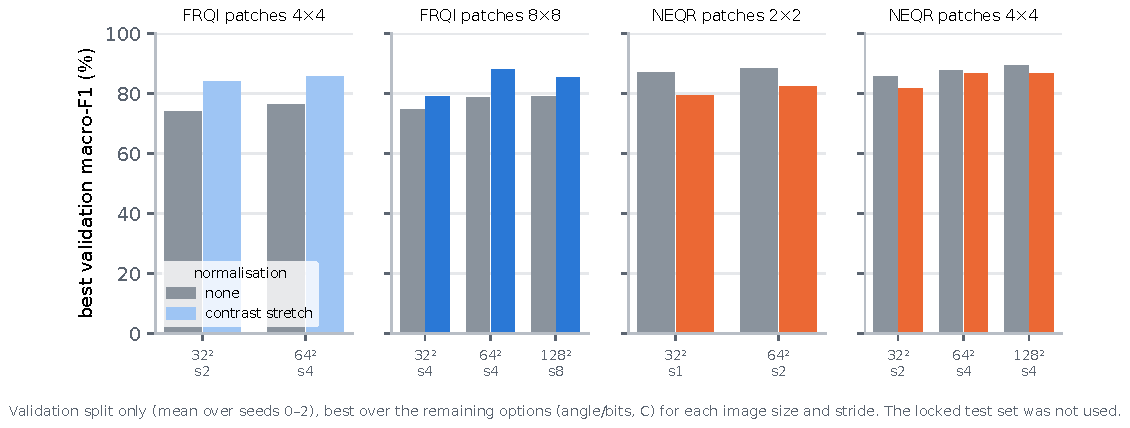
\includegraphics[width=\linewidth]{Fig09_validation_sweep.pdf}
\caption{Validation macro-F1 of the best configuration for each value of the main hyper-parameters, per model group (validation split only; the test set was not used).}
\label{fig:sweep}
\end{figure}

For NEQR the picture differs: without contrast stretch, the best validation macro-F1 is higher ($89.2$ vs.\ $86.8\%$) but its spread across seeds is three times larger ($\pm7.2$ vs.\ $\pm2.3$), a warning sign that is confirmed on the test set below.

\subsection{Error analysis}
Fig.~\ref{fig:cm} shows the confusion matrices of the two headline models, summed over seeds, and Fig.~\ref{fig:perclass} the per-class F1. FRQI is strongest on patches (95.8\%) and crazing (93.1\%). Its two largest error types are inclusion images predicted as pitted surface (38 of 180) and scratches predicted as rolled-in scale (40 of 180), classes whose local patches look alike once global layout is discarded. NEQR loses most on rolled-in scale (65.0\% F1): summed over seeds, it classifies 118 of 180 such test images correctly, whereas FRQI classifies 178.

\begin{figure}[!t]
\centering
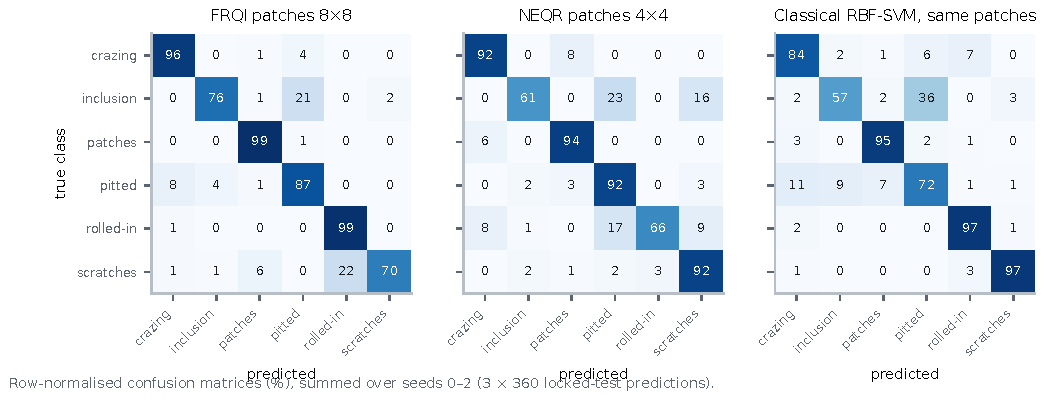
\includegraphics[width=\linewidth]{Fig06_confusion_matrices.pdf}
\caption{Confusion matrices on the locked test set, summed over three seeds, for the FRQI ($8\times8$ patches) and NEQR ($4\times4$ patches) models.}
\label{fig:cm}
\end{figure}

\begin{figure}[!t]
\centering
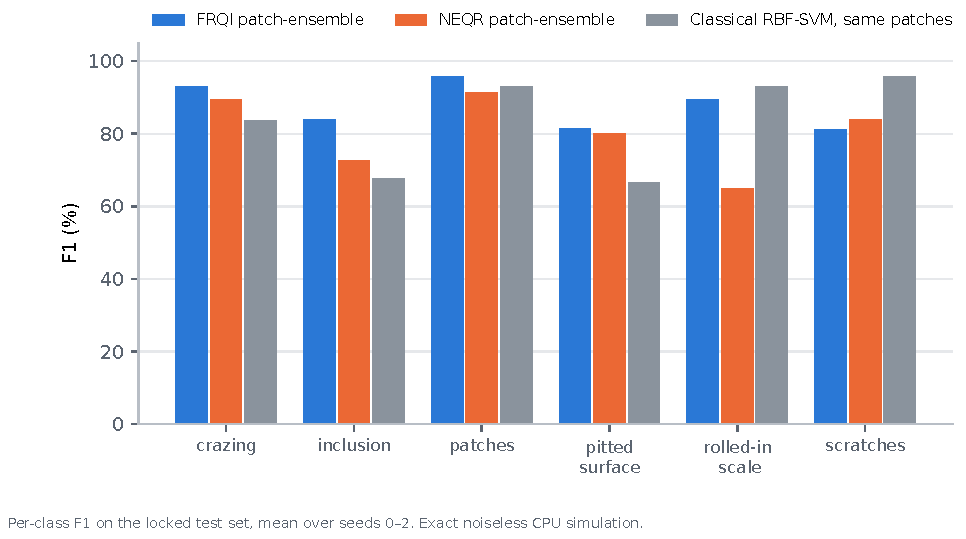
\includegraphics[width=0.9\linewidth]{Fig07_per_class_f1.pdf}
\caption{Per-class F1 on the locked test set (mean over three seeds) for the four patch-ensemble groups and the classical control.}
\label{fig:perclass}
\end{figure}

Fig.~\ref{fig:seeds} explains the large standard deviation of NEQR. Its seed accuracies are 87.5, 71.1 and 89.4\%; on seed~1 it misclassifies every rolled-in-scale test image. The whole-image kernels also struggled with this class, which suggests a brightness shift between the training and test folders for it. FRQI, selected with per-image contrast stretch, is not affected (86.7, 87.2 and 89.4\%). NEQR was not re-tuned after the test, because doing so would use the test set for model choice.

\begin{figure}[!t]
\centering
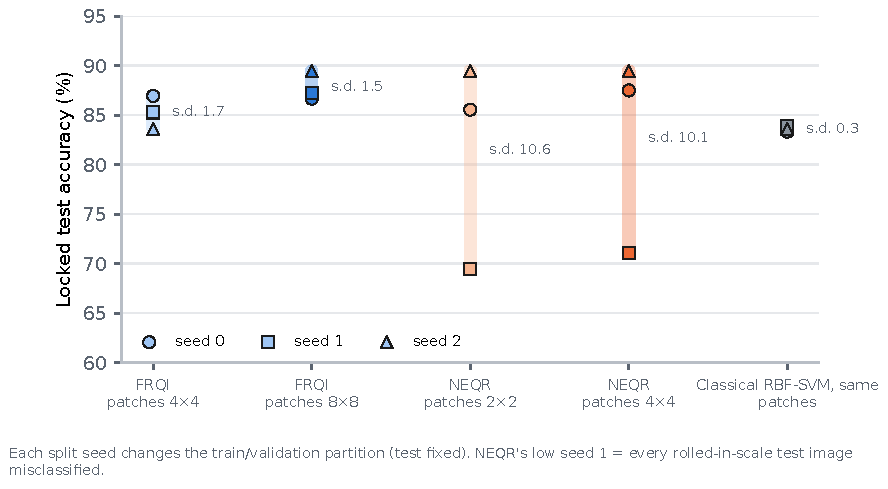
\includegraphics[width=0.8\linewidth]{Fig08_seed_stability.pdf}
\caption{Test accuracy per seed for each V4 group; NEQR drops on seed 1 because of the rolled-in-scale class.}
\label{fig:seeds}
\end{figure}

\subsection{Resources and reconstruction}
One FRQI patch state uses 7 qubits and, after transpilation, 8,339 gates (depth 4,878, 3,584 CX gates); one NEQR patch state uses 8 qubits and 1,998 gates. A swap test between two FRQI patch states would need $2\cdot7+1=15$ qubits, independent of the image size. As shown in Fig.~\ref{fig:recon}, FRQI statevector decoding reproduced all 1,800 images exactly at every resolution; with finite shots the error grows with image size because shots are spread over more pixels (1,000 shots: MSE $8.7\times10^{-3}$ at $8\times8$ and $6.4\times10^{-2}$ at $16\times16$). NEQR is exact up to quantisation (4-bit MSE floor $3.7\times10^{-4}$). For comparison, classical PCA with eight components keeps an SSIM of only 0.59, which helps explain why earlier PCA-input quantum models had little texture to work with.

\begin{figure}[!t]
\centering
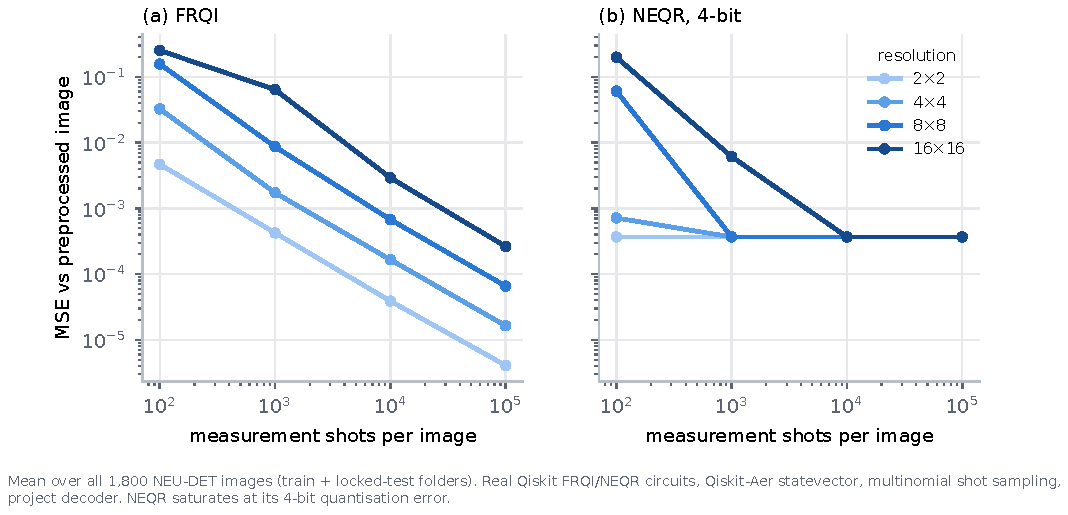
\includegraphics[width=\linewidth]{Fig11_reconstruction_mse_vs_shots.pdf}
\caption{Reconstruction error (MSE, log scale) versus number of measurement shots for whole-image FRQI and NEQR over all 1,800 images; markers show means.}
\label{fig:recon}
\end{figure}

\subsection{Per-image analysis}
To see whether errors are concentrated on a few unusual images, we combined the saved test predictions of all 163 selected models of protocols V2 to V4, each with three seeds. Fig.~\ref{fig:perimage} shows that the median test image is classified correctly by 67\% of the model--seed pairs, that no image is misclassified by every model, and that no image is classified correctly by every model. Averaged over all models, rolled-in scale is the hardest class and patches the easiest, which agrees with the per-class results of the V4 models above. The errors are therefore spread over many images rather than caused by a small set of mislabelled or corrupted samples.

\begin{figure}[!t]
\centering
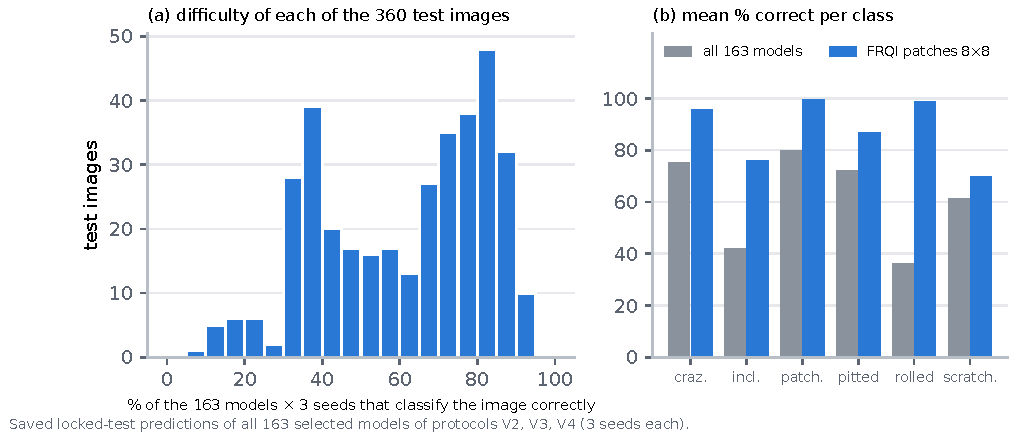
\includegraphics[width=\linewidth]{Fig14_per_image_difficulty.pdf}
\caption{(a) Fraction of all model--seed pairs (163 models of protocols V2--V4, three seeds each) that classify each test image correctly; (b) mean per class, for all models and for the V4 FRQI model.}
\label{fig:perimage}
\end{figure}

% ---------------------------------------------------------------- VII. DISCUSSION
\section{Discussion}
The main lesson is that the low accuracy of FRQI and NEQR kernels on this data was caused by what was being compared, not by the encodings. A whole-image overlap asks whether two images have similar intensities at the same pixels, which is the wrong question for textures. The mixture of patch states asks how often local patterns of one image resemble local patterns of the other, which is much closer to how texture descriptors work. FRQI benefits more than NEQR. A plausible reason is that FRQI overlaps vary smoothly with intensity, especially after contrast stretch and with $b=4$, whereas NEQR overlaps are all-or-nothing for each quantised pixel and are therefore more sensitive to small brightness shifts.

The matched control changes how the result should be read. A classical SVM on the same patches is statistically tied with the FRQI kernel, and every kernel in this study has a closed form that we computed on a laptop. The study therefore shows a better way to use quantum image representations, not a computational advantage. In practice, a hardware version would be attractive mainly because its register size is set by the patch: the FRQI model needs 7 qubits per patch and 15 for a swap test, regardless of image resolution. Its cost is moved into the number of shots, since each kernel entry is a probability that must be estimated, and the differences between kernel entries of different classes can be small.

Several limitations apply. All results come from noiseless simulation, and finite-shot kernel estimation was not simulated for classification. Only one data set was used. The selected SVM parameter $C=1000$ lies at the edge of the grid, so a larger $C$ might have been chosen with a wider grid.

The main threat to validity is that the locked test set is not fresh: it was also used in protocols V2 and V3, and the patch-ensemble idea was proposed after their weak FRQI and NEQR results. Within V4, models were chosen on validation data and tested once, but the choice of method at the protocol level was informed by earlier test results. A few patch geometries were also explored on the validation split before the grid was fixed. Implementation errors were reduced by unit tests that compare the kernel with Qiskit statevectors, and by 17 automated integrity checks of hashes, test accesses and recomputed metrics, all of which pass. The data set contains no personal information, and we see no direct ethical concerns.

% ---------------------------------------------------------------- VIII. CONCLUSION
\section{Conclusion and Future Work}
This paper proposed representing an image by the mixed state of its FRQI- or NEQR-encoded patches and comparing images with the swap-test quantity $\mathrm{Tr}(\rho_A\rho_B)$. For RQ1, the patch-ensemble kernel significantly improves both encodings on NEU-DET: FRQI rises from $60.6\pm1.2\%$ to $87.8\pm1.5\%$ and NEQR from $60.2\pm0.4\%$ to $82.7\pm10.1\%$ ($p<0.001$). For RQ2, the improvement is not attributable to the quantum encoding, since a classical model on the same patches performs equally well ($83.6\pm0.3\%$, $p=0.060$) and a classical texture model remains best ($95.6\pm2.2\%$). The evaluation used validation-only selection, hash-frozen configurations and one test evaluation per model. For practitioners, the main message is that how images are compared matters more than which quantum image encoding is chosen, and that a classical model on the same input should always be reported next to a quantum one. A negative answer to RQ2 is still informative, because it shows where the accuracy actually comes from.

Three directions follow from these results. First, the kernel should be estimated with finite swap-test shots and realistic noise models to measure how many shots are needed for the reported accuracy. Second, the method should be tested on a fresh steel defect data set whose test images have never been used for any design decision. Third, larger patches or entangling encoders could be studied to find out whether patch-ensemble kernels keep their accuracy once they are no longer cheap to simulate classically.

% ---------------------------------------------------------------- DECLARATIONS
\section*{AI-Use Declaration}
A generative AI assistant (Claude, Anthropic) was used to help write and debug the experiment and dashboard code, to generate the figures and tables from our saved results, and to prepare a first draft of the text. The authors reviewed and rewrote the text, checked every number against the result files, and read and verified every reference. All experimental results come from our own runs; none were generated by the AI.

\section*{Contribution Statement}
\noindent Drishti (230527): [EDIT: e.g., method design, quantum encoding and kernel implementation, experiments, paper writing].\\
Abhinav Singh (230528): [EDIT: e.g., data pipeline, classical baselines, dashboard, figures and paper writing].

\bibliographystyle{IEEEtran}
\bibliography{references}
\end{document}
